\documentclass[11pt,titlepage]{article}
\usepackage{Preamble}
\newcommand{\beq}{\begin{equation}}
\newcommand{\eeq}{\end{equation}}
\begin{document}

\begin{titlepage}
    \newgeometry{margin=3cm}
	\centering
    %\includegraphics[width=0.5\linewidth]{epfl.png}\\[0.25cm] 	% University Logo
    %\textsc{\LARGE École Polytechnique Fédérale de Lausanne}\\ \vspace{\fill}
    \textbf{\textsc{\fontsize{50}{50}\selectfont Physique numérique I}}\\ \vspace{\fill}		
	\textsc{\LARGE Spring-pendulum system}\\[0.4cm]
	\rule{\linewidth}{0.2 mm} \\[0.5 cm]
	Baptiste Claudon  -  Kent Barbey\\[0.5cm]Assistant : André Calado Coroado\\[0.5cm]Group 15\\[0.5cm] \today
\end{titlepage}

\thispagestyle{numberonly}



%%%%%%%%%%%%%%%%%%Table des matières et figures%%%%%%%%%%%%%%%%%%
\newpage
\renewcommand\contentsname{\color{black}Table of contents}
\tableofcontents
\vspace{0.5cm}
\begin{invsummary}
\end{invsummary}
\newpage
\listoffigures
\vspace{0.5cm}
\begin{invsummary}
\end{invsummary}
\newpage
%%%%%%%%%%%%%%%%%%%%%%Texte%%%%%%%%%%%%%%%%%%%%%%%%%%%
\section{Introduction}

\newpage
\section{Analytical calculations}
Let us consider the dynamics of a mass $m$ of electric charge $q$ tied to a spring of stiffness $k$ and length at rest $l_0$. The position of the mass over time is given by a vector $\Vec{r}(t)$ in a Cartesian coordinate system with $x$ and $y$ axis as shown in \textbf{Fig.}\ref{lab1}. The spring is attached on its other end to the point $(x,y)=(\widehat{x},\widehat{y})=(0,0)$.
\begin{figure}[H]
    \centering
    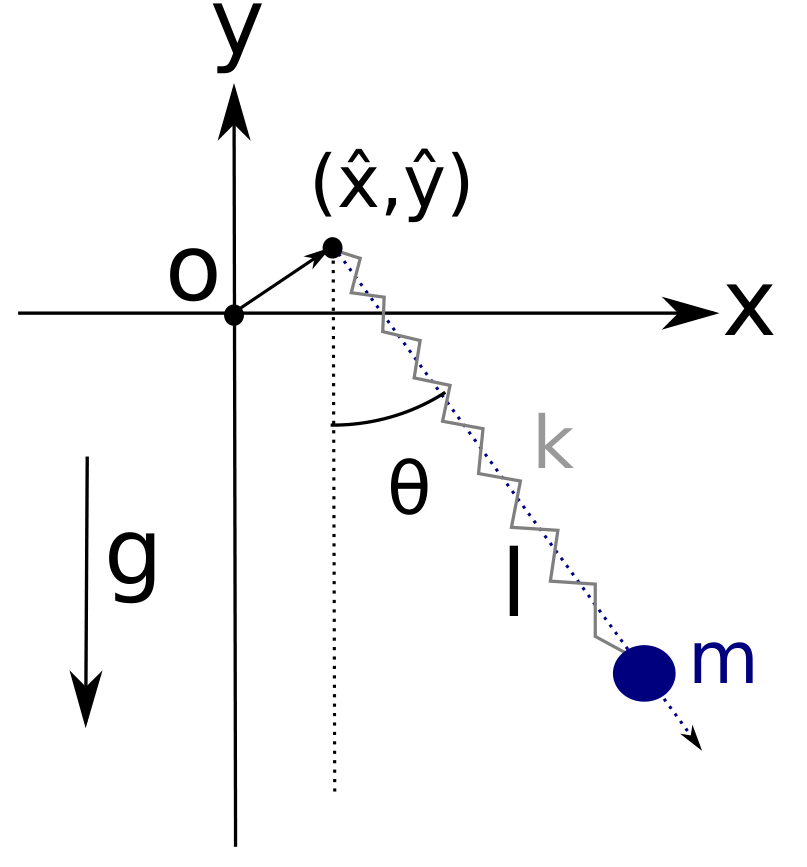
\includegraphics[scale=0.4]{Images/img1.png}
    \caption{Schematic representation of the system }%rajouter reference à l'exo
    \label{lab1}
\end{figure}
The position, speed and acceleration are respectively written as : 
\begin{equation*}
    \Vec{r}(t)=
\begin{pmatrix}
    x(t) \\
    y(t)
\end{pmatrix}
\hspace{3.8cm}
    \Vec{v}(t)=
\begin{pmatrix}
    \dot{x}(t) \\
    \dot{y}(t)
\end{pmatrix}
\hspace{3.8cm}
    \Vec{a}(t)=
\begin{pmatrix}
    \ddot{x}(t) \\
    \ddot{y}(t)
\end{pmatrix}
\end{equation*}
with initial conditions : $x(0)=x_0,\,y(0)=y_0,\,\dot{x}(0)=\dot{y}(0)=0$.\\ \\
The mass is under the influence of four forces :
\begin{enumerate}
    \item The weight : $\Vec{P}= \begin{pmatrix} 0\\-mg \end{pmatrix}$
    \item The spring force : $\Vec{F}_k= \begin{pmatrix} -k(l-l_0)\sin(\theta)\\k(l-l_0)\cos(\theta) \end{pmatrix}$, where $l$ is the length of the spring and $l-l_0$ its deformation.
    \item An oscillating excitation force : $\Vec{F}_E=q\cos(\omega t) \begin{pmatrix} E_x\\E_y \end{pmatrix}$ with $E_{x,y}$ the electric field coordinates and $\omega$ a given frequency.
    \item The drag force : $\Vec{F}_T= -\nu\Vec{v}(t)$
\end{enumerate}
The numerical values for the simulations, unless otherwise stated, are $m=1.5kg$, $k=4.5$N.m$^{-1}$, $l_0=1.1$m, $q=10^{-4}$C and $g=9.81$m.s$^{-2}$.


\subsection{Differential motion equation}
	Noticing that $x=l\sin(\theta)$, $y=-l\cos(\theta)$ and $\theta=				\arctan(\frac{x}{-y})$, Newton's second law yields :
	\begin{equation}
	\vec{F}_k + m\vec{g} + \vec{F}_T + \vec{F}_E = m\vec{a}
	\end{equation}
	Hence the differential equations system :
	\begin{equation}	 
	\left\{
	\begin{array}{l}
		\ddot{x}(t)= -\frac{k}{m}x + \frac{k}{m}l_0\sin(\theta) - \frac{\nu}			{m}\dot{x} + \frac{q}{m}E_x\cos(\omega t) \\ \\
		\ddot{y}(t)= -\frac{k}{m}y - \frac{k}{m}l_0\cos(\theta) - \frac{\nu}			{m}\dot{y} + \frac{q}{m}E_y\cos(\omega t)-g
	\end{array}	
	\right.	 
	\end{equation}
	which is equivalent to :
	\begin{equation}	 
	\left\{
	\begin{array}{l}
		\ddot{x}+\omega_0^2x+\gamma\dot{x}= \omega_0^2l_0\sin(\theta)+					\frac{q}{m}E_x\cos(\omega t) \\ \\
		\ddot{y}+\omega_0^2y +\gamma\dot{y}= - \omega_0^2l_0\cos(\theta) + 				\frac{q}{m}E_y\cos(\omega t)-g
	\end{array}	
	\right.	 
	\end{equation}
	with $\frac{k}{m}=\omega_0^2$ and $\frac{\nu}{m}=\gamma$. These are the 		typical equations of a damped and forced harmonic oscillator.
	

\subsection{Equilibrium}
	Let $E_x=E_y=\nu=0$. Equations (3) are reduced to 
	\begin{equation}
	\left\{
	\begin{array}{l}
	\ddot{x} + \omega_0^2(x-l_0\sin(\theta))=0\\ \\
	\ddot{y} + \omega_0^2(y+l_0\cos(\theta))-g=0
	\end{array}
	\right.
	\end{equation}
	Simple harmonic oscillators equations are recognisable. The equilibrium is determined when the net force is zero, i.e. $\ddot{x}=\ddot{y}=0$. Therefore :
	\begin{equation}
	\left\{
	\begin{array}{l}
	\omega_0^2(x-l_0\sin(\theta))=0\\ \\
	\omega_0^2(y+l_0\cos(\theta))-g=0
	\end{array}
	\right.
	\end{equation}
	The first equation gives two solutions knowing the expressions of $x$ and $y$ in polar coordinates : 
	\begin{enumerate}
	\item $l=l_0$ which is not compatible with the second equation since $g\neq0$.
	\item $\theta_{1,2}=0,\pi$ which gives $x_1=x_2=0$ and by injecting into the second equation : $y_1= -l_0-\frac{g}{\omega_0^2}=-l$ and $y_2=l_0-\frac{g}{\omega_0^2}=l.$
	\end{enumerate}
	Hence the stable and unstable equilibrium positions respectively :
	\begin{enumerate}
	\item $(x_1,y_1)=(0,-l_0-\frac{g}{\omega_0^2})$
	\item $(x_2,y_2)=(0,l_0-\frac{g}{\omega_0^2})$
	\end{enumerate}

\subsection{Mechanical energy}
	By definition, the mechanical energy is given by :
	\begin{equation}
	E_m=E_K+E_P=\dfrac{1}{2}mv^2 + mgy+  \dfrac{1}{2}(l-l_0)^2 -q(E_xx+E_yy)
	\end{equation}
	knowing that : 
	\begin{itemize}
	\item $l=\sqrt{x^2+y^2}$
	\item The electric force being conservative, the electric potential is : 
	$qV=q\left(-\int\vec{E}\vec{dl}\right)=-q(E_xx+E_yy)$ with $\vec{dl}			=(dx,dy)$
	\end{itemize}

\subsection{Non conservative forces' power}
	The only non conservative force is the drag force. By definition, the 			power of a force $\vec{F}_T$ is : 
	\begin{equation}
	P_{nc}=\dfrac{dW_{nc}}{dt} =\dfrac{\vec{F}_T\vec{dr}}{dt}=-\nu v^2
	\end{equation}
	where $v^2=\dot{x}^2 + \dot{y}^2$
\subsection{Small oscillations around the stable solution of the equilibrium}
	Equations (4) is used. Small oscillations $\delta x$ and $\delta y$ are 		applied respectively to $x_1$ and $y_1$. Hence : 
	\begin{gather}
	x(t)=x_1 + \delta x=\delta x \Rightarrow \ddot{x}(t)=\delta\ddot{x}\\
	y(t)=y_1 + \delta y \Rightarrow \ddot{y}(t)=\delta\ddot{y}
	\end{gather}
	Therefore for $\delta x$ : 
	\begin{equation}
	\delta\ddot{x}(t)=-\omega_0^2\delta x - \omega_0^2l_0\sin\left(\arctan\left(\dfrac{x}{y}\right)\right)
	\end{equation}
	A Taylor series expansion around  $x_1$ and $y_1$ gives : 
	\begin{equation}
	-\omega_0^2l_0\frac{d}{dx}\sin\left(\arctan\left(\dfrac{x}{y}\right)\right)\bigg\rvert_{x_1,y_1}\delta x = \frac{\delta x}{y_1}
	\end{equation}
	Hence (11) in (3) yields : 

	\begin{align*}
	\delta\ddot{x}(t)&=-\omega_0^2\delta x\left(1+\dfrac{l_0}{\frac{-g}{\omega_0^2}-l_0}\right)\\
	&=\delta x \dfrac{g}{y_1}\\
	&=\delta x \dfrac{g}{-l_{eq}}
	\end{align*}
	Finally : 
	\begin{equation}
	\delta \ddot{x}(t)+\dfrac{g}{l_{eq}}\delta x=\delta \ddot{x}(t)+\omega_2^2\delta x=0
	\end{equation}
	where $\omega_2^2=\sqrt{\dfrac{g}{l_{eq}}}=\sqrt{\dfrac{kg}{gm+kl_0}}$ the eigenfrequency corresponding to the pendulum. The solution of the initial Cauchy problem(with initial conditions) with (8) is : 
	\begin{equation}
		x(t)=x_0\cos(w_2t)
	\end{equation} 
	
	On the same basis, the equation for a small oscillation for $\delta y$ yields : 
	\begin{align*}
	\delta\ddot{y}(t)&=\omega_0^2(y_1 +\delta y)-\omega_0^2l_0\cos(\theta)-g\\
	&\approx -\omega_0^2(y_1+\delta y) - \omega_0^2l_0-g\\
	&=-\omega_0^2\delta y
	\end{align*}
	Finally the full equation :
	\begin{equation}
	\delta \ddot{y}(t)+\omega_1^2\delta y=0
	\end{equation}
	With $\omega_0^2=\omega_1^2$ and therefore $\omega_1=\sqrt{\dfrac{k}{m}}$ 		the eigenfrequency corresponding to the spring. The solution of the initial Cauchy problem(with initial conditions) with (9) is : 
	\begin{equation}
		y(t)=y_1+\delta y=(y_0-y_1)\cos(\omega_1t)+y_1
	\end{equation}






\newpage
\section{C++ implementation}

\subsection{St\o rmer-Verlet scheme}
\newpage
\section{Simulation and results analysis}

\subsection{Small oscillations around equilibrium : simple harmonic oscillator}

\subsection{Resonance with the exiting force}

\subsection{Large movements without damping nor excitation}

\subsection{Large movements without damping but with excitation}
	
	\subsubsection{Mechanical energy theorem}
	
	\subsubsection{Poincaré maps}
	
	\subsubsection{Sensitivity to initial conditions}
	
\subsection{Large movements with damping and excitation}

	\subsubsection{Mechanical energy theorem}
	
	\subsubsection{Sensitivity to initial conditions : a step towards chaos}
	
	\subsubsection{mah man Poincaré maps}
	
	\subsubsection{Strange attractors}
	
\subsection{To go further...}
\newpage
\section{Conclusion}

\newpage
\section*{Addendum}
% in order to compare with numerical applications and since there are too many parameters to give
%%%%%%%%%%%%%%%%%%%%Style de page%%%%%%%%%%%%%%%%%%%%%
\pagestyle{numberonly}
%%%%%%%%%%%%%%%%%%%%%%%Bibliographie%%%%%%%%%%%%%%%%%%
\printbibliography

\end{document}
